\subsection{Choosing the functions}

The first task is to implement some helper functions for slices, similar as to how they exist
for lists in Haskell. To decide on which functions will be implemented, popular
Haskell repositories on GitHub have been analysed. The popularity of repositories
was decided to be based on their number of stars. Out of all Haskell projects
on GitHub, the most popular are\autocite{github-popular-haskell}:

\begin{itemize}
    \item Shellcheck (koalaman/shellcheck\autocite{github-shellcheck}): A static analysis tool for shell scripts
    \item Pandoc (jgm/pandoc\autocite{github-pandoc}): A universal markup converter
    \item Postgrest (PostgREST/postgrest\autocite{github-postgrest}): REST API for any Postgres database
    \item Semantic (github/semantic\autocite{github-semantic}): Parsing, analyzing, and comparing source code across many languages
    \item Purescript (purescript/purescript\autocite{github-purescript}): A strongly-typed language that compiles to JavaScript
    \item Compiler (elm/compiler\autocite{github-elmcompiler}): Compiler for Elm, a functional language for reliable web apps
    \item Haxl (facebook/haxl\autocite{github-haxl}): A Haskell library that simplifies access to remote data, such as databases or web-based services
\end{itemize}

In these repositories, the number of occurrences of popular list functions has
been counted. The analysis does not differentiate between different `kinds' of
functions. For example, `fold' includes all occurrences of `foldr', `foldl' and
`foldl\''; `map' includes occurrences of `fmap', `mapM' and `mapM\_'.
Also, the analysis has not been done with any kind of AST-parsing.
Rather, a simple `grep' has been used to find matches. This means that it is
likely to contain some mismatches, for example in code comments. All in all,
this analysis should only be an indicator of what functions are used most.

Running the analysis on the 7 repositories listed above, searching for a number
of pre-selected list functions, indicates that the most used functions are `:'
(cons), `map' and `fold', as shown in table~\ref{tab:occurrences-list-funcs}.

\begin{table}[htb]
\centering
\begin{tabular}{ll}
\toprule
`:' (cons) & 2912 \\
\midrule
map & 2347 \\
\midrule
fold & 610 \\
\midrule
filter & 562 \\
\midrule
take & 376 \\
\midrule
drop & 238 \\
\midrule
reverse & 185 \\
\midrule
sum & 173 \\
\midrule
zip & 158 \\
\midrule
product & 56 \\
\midrule
maximum & 53 \\
\midrule
minimum & 26 \\
\end{tabular}
\caption[Occurrences of list functions]{Occurrences of list functions\footnotemark}
\label{tab:occurrences-list-funcs}
\end{table}

\footnotetext{See Appendix~\ref{appendix:function-occurrences} for more information}
%\footnote{The map function listed here also includes occurrences of `fmap'. A more
    %detailed look at the data shows that there are 632 occurrences of `fmap', which
    %means that `fmap' and `map' are used equally as often. As `fmap' however requires
    %some kind of implementation for an `iterable', it is out of scope for this paper.
%}

Based on this information, it has been decided to implement the map, cons, fold
and filter functions into the Go compiler\footnote{The cons function (`:') is overrepresented in this list,
    as it can also be used to deconstruct lists within pattern matching. Filtering
    these occurrences would need a more advanced algorithm. However, even if $\tfrac{3}{4}$
    of these usages are used in pattern matching, the cons function would still be
    in the top 3.
}.

\subsection{Map}

The most used function in Haskell is map. The table~\ref{tab:occurrences-list-funcs}
counts roughly 1200 occurrences of map, although around 600 of those occurrences are from
fmap. fmap is part of the Functor type class\footnote{type classes
    in Haskell are similar to interfaces in imperative and object-oriented
languages}, which is described as `a type that can be mapped over'\autocite{functor-wiki}.
In general, a common analogy of the Functor type class is a box. A functor is like a box
where a value can be put into and taken out again. fmap processes and transforms the item
in that box. For lists, this process means iterating over and processing every item within that list.
For the `Maybe' type it means `unpacking' the concrete value and processing it, or if there is
no concrete value, returning `Nothing' instead.

The map function is exactly like fmap but only works on lists:

\begin{quote}
    \[map\] returns a list constructed by applying a function (the first argument) to all
    items in a list passed as the second argument\autocite{haskell-map}.
\end{quote}

Some usage examples of map can be seen at~\ref{code:haskell-map}.

\begin{listing}
    \begin{haskellcode}
Prelude> :t map
map :: (a -> b) -> [a] -> [b]
Prelude> :t fmap
fmap :: Functor f => (a -> b) -> f a -> f b
Prelude> map (*3) [1,2,3]
[3,6,9]
Prelude> fmap (*3) [1,2,3]
[3,6,9]
Prelude> map (++ " world") ["hello","goodbye"]
["hello world","goodbye world"]
Prelude> map show [1,2,3]
["1","2","3"]
    \end{haskellcode}
    \caption{Example usage for map and fmap}\label{code:haskell-map}
\end{listing}
Due to missing polymorphism, map cannot be implemented easily in Go. While
a specific definition of map would be
\begin{gocode}
func map(f func(int) string, []int) []string
\end{gocode}
this definition would only hold true for the specific type combination \mintinline{go}|int|
and \mintinline{go}|string|. A more generic definition, similar to append,
would be:
\begin{gocode}
func map(f func(Type1) Type2, []Type1) []Type2
\end{gocode}
For this to work, the function has to be implemented as a built-in into the compiler.

As there is already a `map' token in the Go compiler (for the map data type),
the function will be called `fmap'. However, compared to Haskell's `fmap',
Go's `fmap' only works on slices. This is due
to the absence of an `functor'-like concept. Again, due to the absence of polymorphism,
this cannot realistically built into the language.

Nonetheless, to avoid possible naming confusions, the `map' function in Go will
be called `fmap'.

In Go, the usage of `fmap' should result in making the program~\ref{code:fmap-usage-go}
behave as shown\footnote{Printf's first argument, the
verb `\%\#v', can be used to print the type (`\#') and the value (`v') of a
variable\autocite{fmt-godoc}.}.

\begin{listing}
\begin{gocode}
package main

import (
  "fmt"
  "strconv"
)

func main() {
  fmt.Printf("%#v", fmap(strconv.Itoa, []int{1, 2, 3})) // []string{"1", "2", "3"}
}
\end{gocode}
\caption{Example usage of map in Go}\label{code:fmap-usage-go}
\end{listing}
\subsection{Cons}

The name cons has been introduced by LISP, where it describes a record structure
containing two components called the `car' (the `\textbf{c}ontents of the \textbf{a}ddress \textbf{r}egister')
and the `cdr' (`\textbf{c}ontent of \textbf{d}ecrement \textbf{r}egister').
Lists are built upon cons cells, where the `car' stores the element and `cdr' a
pointer to the next cell - the next element of the list.
This is why in Lisp, \mintinline{lisp}|(cons 1 (cons 2 (cons 3 (cons 4 nil))))| is equal to
\mintinline{lisp}|(list 1 2 3 4)|. This list is also visualised in picture~\ref{fig:cons}.

\begin{figure}[h!]
  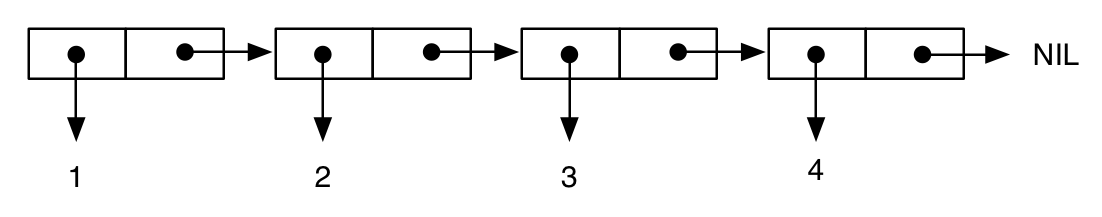
\includegraphics[width=\linewidth]{../img/cons.png}
  \caption{Cons cells forming a list\autocite{cons-image-source}}
  \label{fig:cons}
\end{figure}

The cons operator thus prepends an element to a list, effectively allocating a
variable that contains the newly added element and a pointer to the `old' list.
As a result, prepending to a list is computationally cheap, needing one allocation
and one update.

In Haskell, the `name' of the cons function is the `:' operator.
In Go, names for identifiers (which includes function names) underlie a simple
rule:
\begin{quote}
    An identifier is a sequence of one or more letters and digits. The first
    character in an identifier must be a letter.\autocite{spec-identifiers}
\end{quote}

This rule forbids a function to be named `:'. Instead, the function could be
named `cons'. However, Go already has a function to add to the end of a slice,
`append'. Thus, adding to the beginning of a slice will be named `prepend'.
Using prepend should be very similar to append. The behaviour of `prepend'
should be equal to using `append' with a slight workaround\footnote{This workaround
	is to create a slice containing the prepended element, and expanding the
destination slice with `...', as \mintinline{go}|append| is a variadic function}:

\begin{listing}
    \begin{gocode}
package main

import (
  "fmt"
  "strconv"
)

func main() {
	fmt.Printf("%#v", append([]int{0}, []int{1,2,3}...)// []int{0, 1, 2, 3}
	fmt.Printf("%#v", prepend(0, []int{1, 2, 3})) // []int{0, 1, 2, 3}
}
\end{gocode}
    \caption{Example usage of prepend in go}\label{code:prepend-go}
\end{listing}
\subsection{Fold}\label{sec:fold}

Fold, sometimes also named `reduce' or `aggregate', is another higher-order function
that is very commonly used in functional programming.

\begin{quote}
    analyze a recursive data structure and through use of a given
    combining operation, recombine the results of recursively processing its
    constituent parts, building up a return value.\autocite{fold-wiki}
\end{quote}

In other words, fold processes a list one by one and executes a `combining operation'
on every element, for example summing up a list of integers.

The family of fold functions in Haskell consist of three different implementations of
that definition: foldr, foldl and foldl'.
The difference between foldr and foldl is hinted at their function headers:
\begin{listing}
    \begin{haskellcode}
Prelude Data.List> :t foldl
foldl :: Foldable t => (b -> a -> b) -> b -> t a -> b
Prelude Data.List> :t foldr
foldr :: Foldable t => (a -> b -> b) -> b -> t a -> b
    \end{haskellcode}
    \caption{Function headers of the fold functions}
\end{listing}
The argument with type `b' is passed as the first argument to the foldl
function, and as the second argument to foldr. As can be seen in the illustrations
of foldl and foldr in~\ref{fig:fold}, the evaluation order of the two functions
differ.

\begin{figure}[h!]
    \centering
    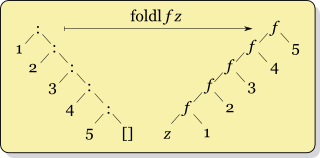
\includegraphics[scale=0.5]{../img/foldl.png}
    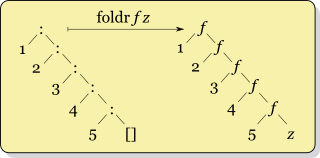
\includegraphics[scale=0.5]{../img/foldr.png}
    \caption{Folds illustrated\autocite{fold-wiki}}
    \label{fig:fold}
\end{figure}

This is most obvious when using an example where the function is not associative:

\begin{listing}
    \begin{haskellcode}
foldl (-) 0 [1..7]
((((((0 - 1) - 2) - 3) - 4) - 5) - 6) - 7 = -28
foldr (-) 0 [1..7]
1 - (2 - (3 - (4 - (5 - (6 - (7 - 0)))))) = 4
    \end{haskellcode}
    \caption{foldr and foldl execution order}\label{code:foldr-example}
\end{listing}
In foldl, the accumulator (`0') is added to the left end of the list (prepended),
while with foldr, the accumulator is added to the right end.
For associative functions (e.g. `+') this does not make a difference, it does
however for non-associative functions, as can be seen in the example~\ref{code:foldr-example}.

The difference between foldl and foldl' is more subtle:
\begin{quote}
    foldl and foldl' are the same except for their strictness properties, so if both
    return a result, it must be the same.\autocite{fold-types}
\end{quote}

The strictness property is only relevant if the function is lazy in its first argument.
If this is the case, behavioural differences can be seen because foldl builds up a so
called `execution path' (nesting the called functions), while foldl' executes these
functions while traversing it already. An example of this is illustrated in
Appendix~\ref{appendix:foldl-strictness}.

To keep things simpler, Go will only have its versions of foldl and foldr, which
will both be strict --- the Haskell counterparts would thus be foldr and foldl'.\footnote{
If the behaviour from the normal foldl function is required, a workaround can
be applied in the Go version. See Appendix~\ref{appendix:foldl-go}}
The usage of these fold-functions is equal to the Haskell versions, where foldl's
arguments are switched in order.

\begin{listing}
\begin{gocode}
package main

import "fmt"

func main() {
  sub := func(x, y int) int { return x - y }
  fmt.Printf("%v\n", foldr(sub, 100, []int{10, 20, 30})) // -80
  fmt.Printf("%v\n", foldl(sub, 100, []int{10, 20, 30})) // 40
}
\end{gocode}
    \caption{Example usage of foldr and foldl in go}\label{code:fold-go}
\end{listing}
\subsection{Filter}

The filter function is the conceptually simplest higher-order function.
It takes a list and filters out all elements that are not matching
a given predicate.
This predicate usually is a function that takes said element and returns
a boolean if it should be kept or filtered.

A simple example:

\begin{listing}
    \begin{gocode}
package main

import "fmt"

func main() {
  smallerThan5 := func(x int) bool {
    return x < 5
  }

  fmt.Println(filter(smallerThan5, []int{1, 8, 5, 4, 7, 3})) // [1, 4, 3]
}
\end{gocode}
    \caption{Example usage of filter in Go}\label{code:filter-go}
\end{listing}
